\documentclass[12pt, a4paper, twoside, openany]{book}
\usepackage[
    a4paper, 
    total={6in, 8in}, 
    top=2cm,
    left=3cm,
    right=2.5cm,
    bottom=1.25cm,
    includeheadfoot,
    headheight=40pt,
]{geometry}
\usepackage[T1]{polski}
\usepackage{graphicx}
\usepackage{fancyhdr}
\usepackage{mathptmx}
\usepackage{enumitem}
\usepackage[utf8]{inputenc}
\usepackage{import}
\usepackage{setspace}
\usepackage{titlesec}
\usepackage{multirow}
\usepackage{longtable}

\import{../}{commands.tex}

\fancypagestyle{plain}{
    \fancyhf{}
    \renewcommand{\headrulewidth}{0pt}
    \fancyhead[C]{\uniimage}
    \fancyfoot[LE,RO]{\thepage}
}

% Wymogi edycyjne: https://moodle2.e-wsb.pl/pluginfile.php/7505508/mod_resource/content/2/Wymogi%20edycyjne_praca%20dyplomowa.pdf

\renewcommand\thesection{\Alph{chapter}\arabic{section}}

\linespread{1.5}

\setlist[itemize]{label=--}

\begin{document}

% Header & footer settings :)
\pagestyle{plain}

\titleformat
{\chapter} %/{〈command 〉}
[block] %/[〈shape〉]
{\bfseries\large} %/ {〈format〉}
{} %/ {〈label 〉}
{0.5ex} %/ {〈sep〉}
{
    \centering
} %/ {〈before-code〉}
{
    \vspace{-0.5ex}%
} %/ {〈after-code〉}

\setcounter{secnumdepth}{4}

\titleformat{\section}[hang]{\normalfont\bfseries}{\thesection.}{0.5em}{}

\titleformat{\subsection}[hang]{\normalfont\bfseries}{\thesubsection.}{0.4em}{}

\titleformat{\subsubsection}[hang]{\normalfont\bfseries}{\thesubsubsection.}{0.4em}{}

\begin{titlepage}
    \begin{center}

        \uniimage

        \MakeUppercase{\department}

        \vspace{5cm}

        \begin{Large} \textbf{\topic} \end{Large}

        \vspace{5cm}

        PROJEKT DYPLOMOWY

        \vfill
        Poznań 2023

    \end{center}
\end{titlepage}

\setcounter{tocdepth}{3}
\tableofcontents

\chapter{\MakeUppercase{dane partnerów}}

\section{Dane Promotora}

\begin{tabular}{ |p{5cm}|p{7cm}|}
    \hline
    Imię i nazwisko         & Izabela Janicka-Lipska \\
    \hline
    Stopień / Tytuł naukowy & dr. inż.               \\
    \hline
    Data i podpis           &                        \\ \hline
\end{tabular}

\section{Dane członków Zespołu projektu}

\membersTable


% Example table and figure formatting
\section{Wprowadzenie}
Lorem ipsum dolor sit amet, consectetur adipiscing elit. Fusce nec justo eu urna accumsan tincidunt. Aliquam erat volutpat.

\chapter{\MakeUppercase{Założenia projektu}}

\section{Opis Projektu}

\subsection{Uzasadnienie wyboru tematu}

Problem utylizacji odpadów stał się w ostatnich latach jednym z największych wyzwań dla społeczeństwa i środowiska naturalnego. Śmieci są produkowane w ogromnych ilościach, a nieprawidłowe postępowanie z nimi prowadzi do skażenia powietrza, wody i gleby. W związku z tym, istnieje potrzeba opracowania rozwiązań, które ułatwią zarządzanie odpadami w sposób bardziej skuteczny i zrównoważony.

Dzięki rozwojowi technologii uczenia maszynowego, pojawiła się możliwość stworzenia aplikacji mobilnej, która rozpoznawać będzie pojemniki na odpady na podstawie zdjęć oraz oznaczać je na mapie. Ułatwi ona lokalizowanie pojemników na dany typ odpadów oraz proces właściwego utylizowania śmieci dla użytkowników. Taka aplikacja może również zwiększyć świadomość społeczną w zakresie utylizacji odpadów i przyczynić się do zmniejszenia ilości odpadów zalegających na składowiskach.


Temat ten jest aktualny i ważny, a jednocześnie daje wiele możliwości na zastosowanie różnych technologii i algorytmów uczenia maszynowego. Przy realizacji projektu można wykorzystać m.in. sieci neuronowe, algorytmy uczenia głębokiego, przetwarzanie obrazów, uczenie maszynowe w chmurze oraz usługi geolokalizacyjne.

Podsumowując, projekt \topic jest uzasadniony ze względu na aktualność i ważność tematu, możliwość wykorzystania najnowszych technologii oraz potencjalne korzyści dla społeczeństwa i środowiska naturalnego.

\subsection{Problem badawczy}

Problemem badawczym jest określenie algorytmów uczenia maszynowego najlepiej nadających się do rozpoznawania pojemników na odpady na podstawie zdjęć oraz określenie cech obrazów odpowiadających za skuteczność modelu.

W ramach tego problemu badawczego można skoncentrować się na kilku podproblemach, m.in.:
\begin{itemize}
    \item analiza dostępnych zbiorów danych:
          \begin{itemize}
              \item znalezienie zbiorów danych do treningu i testowania modelu rozpoznawania pojemników na odpady;
              \item określenie jak są one zdefiniowane oraz jakie informacje zawierają.
          \end{itemize}
    \item wybór odpowiednich algorytmów uczenia maszynowego:
          \begin{itemize}
              \item określenie algorytmów uczenia maszynowego, które najlepiej nadają się do rozpoznawania pojemników na odpady na podstawie zdjęć.
          \end{itemize}
    \item przygotowanie zbiorów danych:
          \begin{itemize}
              \item zastosowanie technik przetwarzania obrazów;
              \item potencjalne użycie technik augmentacji danych.
          \end{itemize}
    \item implementacja i trening modelu: wyłonienie najlepszej techniki trenowania modelu bazowanego na obrazach;
    \item ocena skuteczności modelu: określenie metryk, które pozwolą dokładnie ocenić skuteczność modelu w rozpoznawaniu pojemników na odpady;
    \item analiza cech obrazów: na podstawie analizy modelu, zlokalizowanie cech obrazów odpowiadających za skuteczność procesu rozpoznawania pojemników na odpady;
\end{itemize}

\subsection{Cel główny i cele szczegółowe projektu}

Celem nadrzędnym jest stworzenie aplikacji mobilnej, która będzie pomagać użytkownikom w identyfikacji oraz lokalizowaniu pojemników na odpady danego typu. Aplikacja ta będzie miała na celu wspomaganie procesu utylizacji odpadów w odpowiedzialny i racjonalny sposób poprzez ułatwienie segregacji odpadów oraz zapobieganie ich niewłaściwemu składowaniu.

Cele podrzędne:
\begin{itemize}
    \item analiza dostępnych zbiorów danych: analiza zbiorów danych dostępnych w Internecie, które mogą posłużyć do treningu i testowania modelu rozpoznawania pojemników na odpady;
    \item wybór odpowiednich algorytmów uczenia maszynowego: wybór algorytmów uczenia maszynowego, które będą najlepiej nadawały się do rozpoznawania pojemników na odpady na podstawie zdjęć;
    \item przygotowanie zbiorów danych: przygotowanie zbiorów danych do treningu modelu rozpoznawania pojemników na odpady;
    \item implementacja i trening modelu: implementacja i trening modelu rozpoznawania pojemników na odpady;
    \item ocena skuteczności modelu: ocena skuteczności modelu rozpoznawania pojemników na odpady;
    \item analiza cech obrazów: analiza cech obrazów odpowiadających za skuteczność procesu rozpoznawania pojemników na odpady;
    \item określenie, które cechy obrazów mają największy wpływ na skuteczność procesu rozpoznawania i jak można je wykorzystać do dalszej optymalizacji modelu.
\end{itemize}

\subsection{Zakres podmiotowy, przedmiotowy, czasowy i przestrzenny}

\begin{itemize}
    \item Zakres podmiotowy projektu \topic  obejmuje badanie i opracowanie aplikacji mobilnej oraz algorytmów uczenia maszynowego, które umożliwią rozpoznawanie pojemników na odpady. Podmiotem badania jest zatem aplikacja mobilna Trashify oraz modele uczenia maszynowego, które będą umożliwiać rozpoznawanie pojemników na odpady.
    \item Zakres przedmiotowy obejmuje badanie możliwości rozpoznawania różnych typów pojemników na odpady (np. pojemnik na papier, szkło, plastik, odpady organiczne itp.) oraz opracowanie algorytmów uczenia maszynowego, które umożliwią ich poprawną identyfikację. W ramach projektu będzie również opracowana aplikacja mobilna, która będzie integrować te algorytmy oraz udostępniać użytkownikom informacje o pojemnikach na odpady oraz umożliwiać im łatwe i szybkie ich zlokalizowanie.
    \item Zakres czasowy projektu obejmuje okres od 01.04.2023 aż do 01.12.2023.
    \item Zakres przestrzenny projektu obejmuje miejsce, w którym aplikacja Trashify będzie wykorzystywana, czyli przede wszystkim Polska. Projekt ogranicza się do konkretnego obszaru geograficznego, ponieważ algorytmy uczenia maszynowego, które zostaną opracowane w ramach projektu, będą skupiały się na pojemnikach na odpady spotykanych w Polsce. W ramach projektu nie będzie prowadzona analiza pojemników spotykanych w innych krajach.
\end{itemize}

\subsection{Metody i techniki badawcze}
\begin{itemize}
    \item Metoda analizy i konstrukcji logicznej:
          \begin{itemize}
              \item analiza składników systemu informacyjnego Trashify na składniki cząstkowe (np. interfejs użytkownika, algorytmy uczenia maszynowego, baza danych itp.);
              \item indywidualna analiza każdego z tych składników,
                    synteza wyników analizy w celu stworzenia spójnego i logicznego systemu informacyjnego.
          \end{itemize}
    \item Metoda statystyczna:
          \begin{itemize}
              \item badanie preferencji użytkowników w zakresie korzystania z aplikacji mobilnej Trashify na ograniczonej próbie;
              \item pozyskanie informacji o średniej ilości odpadów segregowanych przez użytkowników korzystających z aplikacji;
              \item analiza zależności pomiędzy poszczególnymi cechami użytkowników a ich zachowaniem w kontekście segregacji odpadów.
          \end{itemize}
    \item Metoda symulacji komputerowej:
          \begin{itemize}
              \item wykorzystanie algorytmów uczenia maszynowego do stworzenia modelu rozpoznającego typ pojemnika na odpady;
              \item przeprowadzenie symulacji na tym modelu, aby zbadać wpływ różnych czynników trafność jego predykcji (np. rozdzielczość zdjęcia, kąt pod jakim zostało ono wykonane, oświetlenie itp.).
          \end{itemize}
    \item Metoda heurystyczna:
          \begin{itemize}
              \item analiza problemów i wyzwań związanych z korzystaniem z aplikacji Trashify i sortowaniem odpadów przez użytkowników;
              \item odkrywanie nowych rozwiązań i podejść do tych problemów;
              \item badanie opinii użytkowników i na ich podstawie wprowadzanie ulepszeń w aplikacji.
          \end{itemize}
\end{itemize}

\section{Ryzyko związane z realizacją projektu}

\begin{enumerate}[label=--]
    \item Ryzyko technologiczne -- związane z wykorzystaniem nowych technologii, które mogą nie działać zgodnie z oczekiwaniami, bądź w trakcie projektowania i implementacji systemu, mogą pojawić się trudności techniczne.
    \item Ryzyko projektowe -- związane z niedostatecznymi planami, wyboru niewłaściwej metodyki lub zła interpretacja wymagań.
    \item Ryzyko jakościowe -- związane z niedostatecznymi testami, błędami w kodzie, które mogą prowadzić do awarii systemu, co może prowadzić do opóźnień w realizacji projektu.
    \item Ryzyko bezpieczeństwa -- związane z atakami cybernetycznymi na system, które mogą prowadzić do utraty danych lub przestojów w działaniu systemu.
\end{enumerate}

\chapter{Realizacja}

\section{Opracowanie projektu}

\subsection{Decyzje architektoniczne}

Na etapie planowania pracy projektowej kluczowym jest dobranie odpowiednich narzędzi
do poszczególnych elementów aplikacji. Z tego względu zespół zdecydował się na stworzenie
dokumentacji decyzji architektonicznych, w których opisano decyzję, plusy oraz minusy wybranch rozwiązań.

\subsubsection{Aplikacja serwerowa}

Aplikacja serwerowa jest kluczowym elementem niemalże każdego projektu aplikacji
internetowej, czy mobilnej. Służy ona jako bezpieczne środowisko do przechowywania danych
użytkowników oraz przeprowadzania skomplikowanych operacji zbyt wymagających i/lub
niebezpiecznych dla środowisk klienckich.

Przy projektowaniu aplikacji kluczowym było dobranie odpowiednich narzędzi do
poszczególnych elementów pracy, takich jak:
\begin{itemize}
    \item Język programowania wykorzystany do projektowania aplikacji;
    \item Framework;
    \item Testy jednostkowe i integracyjne; % - bla bla, dodam;
    \item Testy e2e; %- bla bla, dodam;
    \item Baza danych; %- bla bla, dodam;
    \item Query Buildery bądź dedykowane ORMy; % Info o tym dlaczego są stosowane
\end{itemize}

\paragraph{Język programowania wykorzystany do projektowania aplikacji\\}

Z uwagi na znajomość tego języka wśród członków zespołu wybraliśmy język JavaScript
po stronie aplikacji serwerowej oraz Swift do stworzenia aplikacji mobilnej na
systemy IOS.

Aplikacja serwerowa uruchamiana jest w środowisku uruchomieniowym Node.js, które bazowane jest na
silniku V8 stworzonym przez firmę Google LLC.

\paragraph{Dobór frameworka aplikacji serwerowej}
\subparagraph{Framework serwerowy\\}

Framework jest zestawem dopasowanych narzędzi do stworzenia konkretnego rozwiązania.
W przestrzeni środowiska Node.js na przestrzeni lat pojawiło się ich wiele, bardziej i
mniej znanych. Przypatrzyliśmy się trzem najbardziej popularnym i na bieżąco wspieranym
rozwiązaniom.

\textbf{Express} -- jeden z pierwszych frameworków dla środowiska Node.js, powstały w roku 2010.
Jest on dojrzałym, niezwykle lubianym przez społeczność rozwiązaniem, oferującym
minimalistyczny interfejs, bezstronny względem wzorców projektowych. Posiada bogaty ekosystem
oprogramowań pośredniczących tworzonych i wspieranych przez społeczność.
Jest on pobierany średnio 13 milionów razy w tygodniu, co czyni go liderem w popularności.

\textbf{Fastify} -- framework zainspirowany Express oraz Hapi. Tak jak w przypadku Expressa,
jest on minimalistyczny, jednakże wprowadza kilka usprawnień oraz rozszerzeń do
konceptów w nim prezentowanych. Głównym wzorcem tego frameworka jest bogaty system
wtyczek, które zaimplementowane są na podstawie skierowanego grafu acyklicznego (Rysunek~\ref{fig:ADG}).
Każda ścieżka żądania HTTP, dekoratory, haki są traktowane jako wtyczki.
Pozwala to na pełną enkapsulację logiki oraz zwiększa bezpieczeństwo aplikacji.

% TODO: Fix numbering
\begin{figure}[h]
    \caption{Reprezentacja skierowanego grafu acyklicznego}
    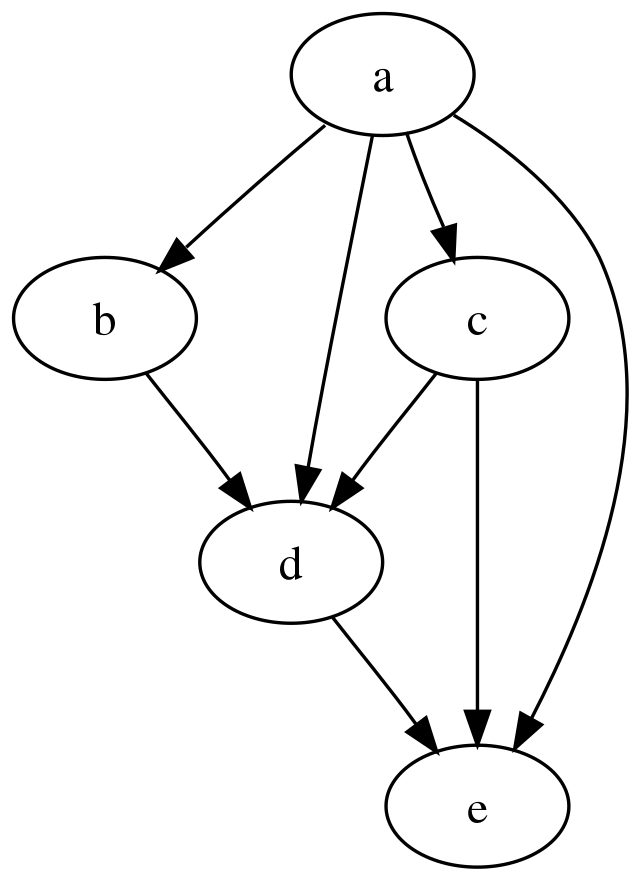
\includegraphics[width=6cm]{../ADG.png}
    \centering
    \label{fig:ADG}
\end{figure}

\textbf{NestJS} -- To framework opiniowany i jako taki wymusza na użytkowniku stosowanie określonych wzorców.
Wykorzystuje progresywny JavaScript, jest zbudowany i w pełni obsługuje TypeScript oraz łączy elementy
programowania obiektowego, programowania funkcyjnego i reaktywnego programowania funkcyjnego.
W przypadku aplikacji internetowych Nest używa Express jako sterownika HTTP,
z opcjonalną konfiguracją Fastify. Zapewnia abstrakcję nad frameworkami,
ale jednocześnie udostępnia ich interfejsy API bezpośrednio programistom, zapewniając uncję wolności.
Jest dostarczany z dedykowanym interfejsem terminalowym, którego można użyć do uruchomienia projektu,
utworzenia nowego z zainstalowanymi wszystkimi zależnościami, generowania zasobów HTTP,
kontrolerów, usług, obiektów transferu danych i innych.

\subparagraph{Decyzja\\}

Zespół projektowy zdecydował się na wykorzystanie frameworka NestJS z wykorzystaniem
Fastify jako sterownik HTTP z uwagi na znaczną różnicę w wydajności względem sterownika Express.

Plusy oraz minusy takiej decyzji są następujące:

\begin{itemize}
    \item gotowa do wykorzystania architektura aplikacji;
    \item olbrzymia społeczność, od której można czerpać wiedzę na temat rozwiązań 
    oraz korzystać z gotowych rozwiązań popularnych problemów;
    \item mniejsza ilość kodu bazowego do napisania;
    \item prostsza separacja logiki biznesowej;
    \item ułatwione testowanie jednostkowe oraz integracyjne za pomocą wstrzykiwaniu
    zależności oraz wbudowanym narzędziom testowym;
    \item problematyczna implementacja rozwiązań nieprzewidzianych przez twórców
    frameworka;
    \item niski poziom kontroli nad cyklem życia żądań HTTP oraz samej architektury;
    \item komunikaty błędów mogą niewiele mówić programiście, co utrudnia proces debuggowania.
\end{itemize}

\paragraph{Dobór frameworka do testowania automatycznego}
\subparagraph{Testowanie aplikacji\\}

Testowanie aplikacji jest kluczową decyzją dla zespołu programistów.
Chociaż początkowo może to być uważane za stratę czasu, umożliwia ono pewniejsze rozwijanie kodu, uniknianie błędów i łatwiejsze zrozumienie kodu źródłowego (z testami będącymi rodzajem dokumentacji w kodzie opisującej zachowanie danej funkcjonalności).
Zespół postanowił rozejrzeć się za opcjami i na myśl przyszły dwie najpopularniejsze: Jest oraz Mocha + Chai.

\textbf{Jest} -- popularny i pełen wbudowanych funkcjonalności framework testowy JavaScript używany głównie do testów jednostkowych stworzony przez firmę Facebook (obecnie Meta). Główne możliwości Jesta są następujące:
\begin{enumerate}[label=--]
    \item Łatwa konfiguracja - w pliku `package.json`, plikach `.jest` lub `jest.js`. Dodatkowo, konfiguracje mogą być dostosowane do konkretnych scenariuszy i stosowane dynamicznie przez program uruchamiający testy;
    \item Obsługa różnych typów testów, takich jak testy jednostkowe, integracyjne, e2e z dodatkiem bilbioteki supertest i testów migawkowych;
    \item mocking - z wysokim stopniem dostosowania, w tym mockowanie wartości zwracanych (zarówno w funkcjach synchronicznych, jak i asynchronicznych). Są one przechowywane i mogą być walidowane;
    \item pokrycie kodu - wbudowane narzędzie do raportowania pokrycia kodu źródłowego;
    \item testowanie równoległe - zwiększenie szybkości testowania, zwłaszcza gdy testy są w pełni niezależne i nie mutują wspólnego zestawu danych;
    \item tryb watch - uruchamianie testów w tle wraz ze zmianami w kodzie źródłowym i/lub samych testach;
    \item test matchers - wbudowany zestaw matcherów, które pozwalają na szybkie i wygodne sprawdzanie wyników funkcji i/lub komponentów. Obejmują one między innymi: `toEqual`, `toHaveLength`, `toContain`, `toBeTruthy`, `toBeDefined`;
    \item konfiguracja globalna - możliwość zadeklarowania zestawu akcji lub manipulacji przed wszystkimi testami (lub określonym ich podzbiorem). Pozwala to programiście na zbudowanie konkretnego, czasochłonnego modułu lub funkcjonalności raz i operowanie na nim we wszystkich testach. Hooki zadeklarowane w konfiguracji globalnej zostaną zastosowane do wszystkich zestawów testów;
    \item obsługa globalnego usuwania środowiska;
    \item haki cyklu życia testów - są to `beforeEach()`, `beforeAll()`, `afterEach()` i `afterAll()`, które pozwalają na wykonywanie akcji w określonych punktach uruchomionych testów. Pozwala to programistom zadeklarować takie akcje raz i zastosować je do wszystkich przypadków;
    \item wsparcie dla środowisk testowych Node.js i przeglądarki;
    \item jednoczesne uruchamianie testów w danej przestrzeni (funkcja eksperymentalna).
\end{enumerate}

\textbf{Mocha z Chai} -- framework testowy Mocha z biblioteką do asercji Chai:
\begin{enumerate}[label=--]
    \item wyczerpujące i czytelne dla człowieka asercje;
    \item używane głównie w BDD (Behavior-Driven Development);
    \item obsługa haków cyklu życia `before`, `after`, `beforeEach` i `afterEach`;
    \item testowanie równoległe ma swoje dobrze zdefiniowane ograniczenia, takie jak użycie `it.only` lub `describe.only`, które są niedostępne. Testowanie równoległe jest dostępne tylko w środowisku Node.js. Haki zadeklarowane na poziomie root nie są globalne w przypadku testowania równoległego;
    \item dostępny cały zestaw reporterów, zarówno wbudowanych, takich jak `json-stream`, `markdown`, `progress`, `xunit`, `html reporter`, jak i opcji innych firm. Nie działają one dobrze z testami równoległymi, ponieważ oczekują, że Mocha będzie wiedzieć, ile testów planuje uruchomić przed wykonaniem;
    \item obsługa globalnej konfiguracji za pomocą `mochaGlobalSetup`;
    \item obsługa globalnego usuwania środowiska za pomocą `mochaGlobalTeardown`;
    \item obsługa zarówno modułów ES, jak i CommonJS, z zastrzeżeniem, że moduły ES nie są obsługiwane przez tryb watch. To samo dotyczy niestandardowych raportów i niestandardowego interfejsu;
    \item konfiguracja może być tylko plikiem CommonJS `.mocharc.js` lub `.mocharc.cjs`.
\end{enumerate}

\subparagraph{Decyzja\\}

Zespół zdecydował się na framework testowy Jest, ponieważ nie wymaga wielu dodatkowych wtyczek do spełnienia potrzeb zespołu. Ponadto ma lepsze wsparcie dla testów równoległych i posiada potężny zestaw funkcji, które umożliwią szybsze tworzenie pakietów testowych.

Plusy oraz minusy takiej decyzji są następujące:
\begin{itemize}
    \item Testy będą tworzone przy użyciu dobrze ugruntowanych reguł;
    \item Pakiet jest-plugin będzie musiał zostać dodany do pliku `.eslintrc` i `package.json`.
    \item Jest ma olbrzymią społeczność z dużą ilością ekspertów, którzy go używają i otwarcie dzielą się wiedzą.
    \item Ilość matcherów i funkcjonalności może stać się przytłaczająca i prowadzić do mniejszej produktywności.
\end{itemize}

\paragraph{Dobór bazy danych}

\subparagraph{Typy baz danych\\}

\textbf{Bazy nierelacyjne -- Not only SQL (NoSQL)}:\\
Bazy danych No-SQL nie mają tak sztywnego schematu bazy danych jak ich relacyjne odpowiedniki. Struktura organizacyjna różni się w zależności od typu nierelacyjnej bazy danych. Biorąc to pod uwagę, wszystkie mają na celu rozwiązanie problemów tradycyjnej, relacyjnej bazy danych, poprzez rozwiązanie kwestii elastyczności i skalowalności. Bazy danych SQL nie są idealne do przechowywania nieustrukturyzowanych formatów danych, takich jak tekst, wideo i obrazy. Bazy danych NoSQL przedkładają dostępność nad spójność.
Termin NoSQL nie oznacza, że dana baza danych nie obsługuje poleceń SQL (niektóre obsługują SQL), można go dokładnie podsumować jako ,,nie tylko SQL``.
Rodzaje nierelacyjnych struktur baz danych to:
\begin{enumerate}[label=--]
    \item Key-value store - jest to model bez schematu, w którym dane są zorganizowane w słownik par klucz-wartość, gdzie każdy element ma klucz i wartość. Klucz może być podobny do tego, co znajduje się w relacyjnej bazie danych, np. identyfikator koszyka, podczas gdy wartości są tablicą danych, np. każdy pojedynczy element w koszyku użytkownika. Są one powszechnie stosowane w systemach o dużej objętości, które wymagają najszybszego możliwego czasu reakcji. Ze względu na nieodłączną strukturę danych, nie są one idealne, gdy trzeba odzyskać wiele rekordów na raz. Przykładami takich baz danych są Redis i Memcached.
    \item Document store - jak sama nazwa wskazuje, są to bazy danych, w których przechowywane są obiekty podobne do dokumentów. Dane przechowywane w takiej bazie danych są zwykle zorganizowane w formacie częściowo ustrukturyzowanym, takim jak JSON, XML lub BSON. Daje to programistom większą elastyczność, ponieważ schematy danych nie muszą dokładnie odpowiadać wzorcom innych dokumentów przechowywanych w danej kolekcji. Złożone transakcje mogą być jednak problematyczne i prowadzić do uszkodzenia danych. Popularne przypadki użycia baz danych dokumentów obejmują systemy zarządzania treścią i profile użytkowników. Przykładem bazy danych zorientowanej na dokumenty jest MongoDB.
    \item Wide-column store - informacje są przechowywane w kolumnach, co pozwala użytkownikom uniknąć nadmiernego i niedostatecznego pobierania, ograniczając alokację pamięci. Ta baza danych próbuje rozwiązać niedociągnięcia magazynów klucz-wartość i dokumentów, ale ponieważ może być bardziej złożonym systemem do zarządzania, nie jest zalecana do stosowania w nowszych zespołach i projektach. Apache HBase i Apache Cassandra są przykładami baz danych o otwartym kodzie źródłowym i szerokim zakresie kolumn. Apache HBase jest zbudowany na bazie Hadoop Distributed Files System, który zapewnia sposób przechowywania rzadkich zestawów danych, co jest powszechnie stosowane w wielu aplikacjach big data. Z kolei Apache Cassandra została zaprojektowana do zarządzania dużymi ilościami danych na wielu serwerach i w klastrach obejmujących wiele centrów danych. Jest ona wykorzystywana w różnych przypadkach, takich jak serwisy społecznościowe i analiza danych w czasie rzeczywistym.
    \item Graph store - zwykle używany do przechowywania grafu wiedzy, w którym elementy danych są przechowywane jako węzły, krawędzie i właściwości. Węzłem może być dowolny obiekt, miejsce lub osoba. Krawędź definiuje relację między węzłami. Grafowe bazy danych służą do przechowywania i zarządzania siecią połączeń między elementami w ramach grafu. Neo4j, oparta na grafach usługa bazodanowa oparta na Javie z edycją społecznościową open source, w której użytkownicy mogą kupować licencje na tworzenie kopii zapasowych online i rozszerzenia wysokiej dostępności lub licencjonowaną wersję wstępną z kopią zapasową i rozszerzeniami.
\end{enumerate}

Teoria CAP \\
Tak zwana ,,teoria CAP`` oznacza spójność, dostępność lub tolerancję partycji. Relacyjne bazy danych zapewniają, że informacje są zawsze zsynchronizowane i spójne. Nie jest tak w przypadku baz danych takich jak Redis, ponieważ wolą one zawsze zapewniać odpowiedź. Oznacza to, że informacje otrzymane z zapytania mogą być nieprawidłowe o kilka sekund - być może nawet do pół minuty. Większość baz danych NoSQL pozostaje zgodna z ,,twierdzeniem CAP``, a nawet jest zgodna z ACID.

\textbf{Relacyjne bazy danych -- SQLowe bazy danych}:\\
\subparagraph*{SQL\\}
Wynaleziony przez Dona Chamberlina i Raya Boyce'a w IBM, SQL jest standardowym językiem programowania do interakcji z systemami zarządzania relacyjnymi bazami danych. Pierwotnie znany jako SEQUEL, został później uproszczony do SQL, ze względu na kwestię znaku towarowego. Jest to de facto standard relacyjnych systemów baz danych. Jak sama nazwa wskazuje, jest to język zapytań, który służy jako pomost między bazą danych a użytkownikami. Niezależnie od tego, czy jest to programista stojący za danym systemem, czy zwykły użytkownik, wszyscy ludzie zaznajomieni z nowoczesną technologią, nawet jeśli nieświadomie, używali SQL. Biorąc pod uwagę, jak blisko relacyjne bazy danych są powiązane z SQL, są one powszechnie nazywane ,,bazami danych SQL``

\subparagraph{Relacyjne bazy danych\\}
Relacyjna baza danych to, jak sama nazwa wskazuje, magazyn danych, który przechowuje je w sposób relacyjny.
Ten typ pamięci masowej rozumie i przechowuje dane w formacie tabelarycznym, tj. wierszy i kolumn.
Relacje są deklarowane za pomocą kluczy podstawowych i obcych, które służą jako identyfikatory danej relacji.
Relacje te są zwykle ilustrowane za pomocą różnych typów modeli danych (https://www.ibm.com/topics/relational-databases).
Kolumny są traktowane jako pola przechowujące nazwę danej zmiennej (na przykład identyfikatorUżytkownika) i typ SQL, podczas gdy wiersze przechowują rzeczywiste wartości.
Relacyjne bazy danych są również zwykle powiązane z transakcyjnymi bazami danych, które uruchamiają polecenia w sekwencji znanej jako transakcja.
Wspomniana transakcja pozwala na przywrócenie zmian, gdy wystąpił błąd w dowolnym kroku procesu.\\
Transakcje mają specyficzne właściwości, które są reprezentowane przez akronim ACID:
\begin{enumerate}[label=--]
    \item \textbf{Atomiczność} - wszystkie zmiany danych są wykonywane tak, jakby były pojedynczą operacją. Oznacza to, że wszystkie zmiany są wykonywane lub żadna z nich nie jest wykonywana.
    \item \textbf{Spójność} - dane pozostają w spójnym stanie od stanu do końca, wzmacniając integralność danych.
    \item \textbf{Izolacja} - stan pośredni transakcji nie jest widoczny dla innych transakcji, w wyniku czego transakcje, które działają jednocześnie, wydają się być serializowane.
    \item \textbf{Trwałość} - po pomyślnym zakończeniu transakcji zmiany w danych utrzymują się i nie są cofane, nawet w przypadku awarii systemu.
\end{enumerate}


\subparagraph*{Decyzja}

Ponieważ projekt będzie w większości dotyczył przechwytywania i przetwarzania obrazów, jedynym realnym i efektywnym czasowo rozwiązaniem będzie system baz danych NoSQL zorientowany na dokumenty.

Plusy oraz minusy takiej decyzji są następujące:
\begin{enumerate}[label=--]
    \item zespół będzie miał większą elastyczność wprowadzania zmian;
    \item obsługa formatów multimediów będzie znacznie prostsza i wykonalna;
    \item zgodność z ACID będzie musiała zostać dokładnie zbadana i wdrożona;
    \item zespół będzie musiał zapoznać się z nową składnią, w zależności od wybranego systemu bazy danych, aby dostosować się do braku znajomości SQL.
\end{enumerate}
% Teoria - warum, co, gdzie, z kim?

% Narzędzia - decyzja, dlaczego?

\subsubsection{Aplikacja mobilna}

\subparagraph{Wybór technologii}
Jako zespół programistów stanęliśmy przed wyborem odpowiedniej technologii do stworzenia aplikacji mobilnej. Przy podejmowaniu decyzji musimy wziąć pod uwagę nasze umiejętności, okres czasu, w którym projekt musi zostać stworzony oraz możliwość wdrożenia niezbędnych funkcjonalności.

\textbf{Javascript -- Ionic 6\\}

Ionic 6 to framework typu open-source do tworzenia aplikacji mobilnych i desktopowych przy użyciu języków programowania sieciowego, takich jak HTML, CSS i JavaScript. Bazuje on na platformie Angular i wykorzystuje komponenty UI oparte na bibliotece Ionic, pozwalając na tworzenie atrakcyjnych i responsywnych aplikacji. Ionic 6 oferuje wiele wbudowanych funkcjonalności i narzędzi, które ułatwiają proces tworzenia i wdrażania aplikacji.
    
Zalety:

- Łatwość i szybkość tworzenia aplikacji dzięki wykorzystaniu języków programowania webowego, takich jak HTML, CSS i JavaScript
- Możliwość tworzenia natywnych aplikacji mobilnych na różne platformy, w tym iOS i Android, a także aplikacji desktopowych
- Duża społeczność deweloperów i rozwijająca się platforma, co oznacza, że istnieje wiele narzędzi, wtyczek i bibliotek, które ułatwiają proces tworzenia aplikacji.
- Wbudowane narzędzia do testowania i debugowania kodu, co ułatwia proces tworzenia i utrzymywania aplikacji
- Dostęp do wielu wbudowanych komponentów UI opartych na bibliotece Ionic, co pozwala na tworzenie atrakcyjnych i responsywnych aplikacji.

Wady:

- W porównaniu do innych popularnych frameworków, takich jak React Native czy Flutter, aplikacje Ionic 6 mogą cechować się gorszą wydajnością ze względu na wykorzystanie technologii webowych
- Brak w pełni natywnej wydajności, co może wpływać na szybkość działania aplikacji, szczególnie w przypadku bardziej złożonych aplikacji
- Możliwe trudności w dostosowaniu aplikacji do różnych platform, co może wymagać dodatkowych prac programistycznych.

\textbf{Javascript -- React Native\\}

React Native to oparty na JavaScript framework do tworzenia aplikacji mobilnych, który umożliwia programistom tworzenie natywnych aplikacji mobilnych na platformy iOS i Android przy użyciu jednej bazy kodu.
Opiera się on na bibliotece ReactJS i wykorzystuje kombinację JavaScript i natywnego kodu do tworzenia wysokowydajnych aplikacji mobilnych.
React Native pozwala programistom na ponowne wykorzystanie kodu na różnych platformach, co pomaga zaoszczędzić czas i zasoby.

Zalety:
\begin{enumerate}[label=--]
    \item Szybkie tworzenie aplikacji dzięki wykorzystaniu JavaScript i popularnej biblioteki React
    \item Możliwość tworzenia natywnych aplikacji mobilnych z jedną bazą kodu dla różnych systemów operacyjnych
    \item Łatwa konserwacja i skalowalność aplikacji dzięki wykorzystaniu komponentów UI wielokrotnego użytku, które mogą być używane w różnych systemach operacyjnych
    \item Dostęp do natywnych funkcji systemu operacyjnego poprzez architekturę "bridge"
    \item Łatwe wdrażanie aktualizacji i zmian aplikacji bez konieczności weryfikacji w sklepie z aplikacjami, która jest wymagana w przypadku aplikacji natywnych
    \item Duża społeczność deweloperów i liczne zasoby online, które ułatwiają rozwiązywanie problemów i znajdowanie gotowych rozwiązań.
\end{enumerate}

Wady:
\begin{enumerate}[label=--]
    \item Niższa wydajność w porównaniu do natywnych aplikacji mobilnych, zwłaszcza w przypadku bardziej złożonych i wymagających aplikacji
    \item Niektóre natywne funkcjonalności mogą być trudne lub niemożliwe do osiągnięcia w React Native, co może wymagać stworzenia dodatkowego natywnego kodu.
    \item Potrzeba znajomości natywnych systemów operacyjnych i ich różnic w celu tworzenia zoptymalizowanych aplikacji dla każdej platformy.
    \item Wyższa krzywa uczenia się dla początkujących programistów, którzy muszą nauczyć się zarówno JavaScript, jak i architektury React Native.
\end{enumerate}

\textbf{Flutter\\}

Flutter to framework open-source do tworzenia aplikacji mobilnych opracowany przez Google. Wykorzystuje on język programowania Dart, który zapewnia szybkość i wydajność, a także zaawansowane narzędzia deweloperskie i obsługę wielu platform. Flutter pozwala na tworzenie aplikacji mobilnych z eleganckimi i atrakcyjnymi interfejsami użytkownika oraz oferuje wiele wbudowanych funkcjonalności i bibliotek, które sprawiają, że tworzenie aplikacji jest szybkie i łatwe.
    
Zalety:
\begin{enumerate}[label=--]
    \item Szybkość i wydajność aplikacji dzięki wykorzystaniu języka programowania Dart oraz implementacji narzędzi Ahead of Time (AOT) i Just in Time (JIT) do kompilacji kodu
    \item Możliwość tworzenia natywnych aplikacji mobilnych na różne platformy, w tym iOS i Android, a także aplikacji webowych i desktopowych
    \item Możliwość tworzenia pięknych i atrakcyjnych interfejsów użytkownika z wykorzystaniem biblioteki Material Design oraz narzędzi do tworzenia animacji i efektów wizualnych
    \item Szybkie wdrażanie zmian i aktualizacji dzięki narzędziom Hot Reload, które pozwalają na szybkie testowanie i modyfikowanie kodu bez ponownego uruchamiania aplikacji
    \item Wbudowane narzędzia do testowania i debugowania kodu, co ułatwia proces tworzenia i utrzymania aplikacji.
\end{enumerate}

Wady:
\begin{enumerate}[label=--]
 \item Mniejsza społeczność deweloperów w porównaniu do innych popularnych frameworków, takich jak React Native czy Ionic
 \item Nieco większe rozmiary plików aplikacji ze względu na wykorzystanie wbudowanych bibliotek i narzędzi
 \item Brak w pełni natywnej wydajności w porównaniu do aplikacji napisanych w językach natywnych, takich jak Java lub Kotlin dla Androida i Objective-C lub Swift dla iOS. Jednak dzięki wykorzystaniu silnika Flutter, który jest zoptymalizowany pod kątem wydajności, różnica w wydajności nie jest tak duża, jak mogłoby się wydawać.
\end{enumerate}

\textbf{Swift\\}
%TODO: PRZEROBIĆ
Programowanie aplikacji mobilnych przy użyciu języków natywnych odnosi się do tworzenia aplikacji przy użyciu języków i narzędzi dostarczanych przez platformę, dla której aplikacja jest tworzona. Na przykład aplikacje na iOS mogą być pisane w języku Swift lub Objective-C, podczas gdy aplikacje na Androida mogą być pisane w języku Kotlin lub Java.
    
Zalety:

- Wysoka wydajność: Aplikacje natywne mają dostęp do pełnych możliwości platformy, co może skutkować szybszym i płynniejszym działaniem w porównaniu do aplikacji zbudowanych przy użyciu wieloplatformowych frameworków.
- Lepsze doświadczenie użytkownika: Aplikacje natywne mogą wykorzystywać komponenty interfejsu użytkownika specyficzne dla platformy, co zapewnia bardziej dopracowane i płynne wrażenia użytkownika.
- Dostęp do funkcji urządzenia: Twórcy aplikacji natywnych mają dostęp do funkcji i możliwości specyficznych dla urządzenia, takich jak GPS, kamera i mikrofon, co pozwala im tworzyć aplikacje z zaawansowanymi funkcjami.
- Solidne narzędzia deweloperskie: Zarówno iOS, jak i Android zapewniają kompleksowe narzędzia programistyczne, w tym zintegrowane środowiska programistyczne (IDE), narzędzia do debugowania i struktury do testowania aplikacji.

Wady:

- Dłuższy czas programowania: Tworzenie aplikacji przy użyciu języków natywnych może być czasochłonnym procesem, ponieważ programiści muszą pisać oddzielne bazy kodu dla każdej platformy.
- Ograniczona przenośność: Aplikacje natywne są powiązane z konkretną platformą, co może ograniczać możliwość ich przenoszenia na inne platformy.
- Stroma krzywa uczenia się: Nauka natywnych języków i narzędzi programistycznych może być trudnym i czasochłonnym procesem, szczególnie dla programistów, którzy są nowicjuszami w tworzeniu aplikacji mobilnych.

\textbf{Decyzja\\}

Zdecydowaliśmy się na wykorzystanie natywnego dla systemów iOS języka Swift ze względu na wbudowane wsparcie Machine Learning oraz możliwość użycia Neural Engine na urządzeniach mobilnych.

\textbf{Konsekwencje\\}

Decyzja o użyciu Fluttera podczas tworzenia aplikacji mobilnej będzie miała kilka pozytywnych konsekwencji. Doprowadzi to do bardzo dobrej wydajności naszej aplikacji. Nasze rozwiązanie będzie dostępne dla urządzeń z systemem Android i IOS. W tym celu będziemy mogli użyć tylko jednego kodu bez konieczności pisania oddzielnych aplikacji. Dzięki wsparciu CoreML unikniemy wielu problemów związanych z implementacją rozwiązania.

Referencje

Teoria - warum, co, gdzie, z kim?

Narzędzia - decyzja, dlaczego?

\subsection{Założenia teoretyczne}

\subsection{Opis sytuacji faktycznej}

\subsection{Badania empiryczne/Inne}

\section{Zadania w projekcie}

\newpage

\begin{longtable}{ | p{0.2\textwidth}| p{0.4\textwidth}| p{0.3\textwidth}| }
    \hline
    Cele szczegółowe projektu & Zadania w projekcie oraz termin rozpoczęcia i zakończenia realizacji zadania                                                                                    & Osoby zaangażowane w realizację zadania \\
    \hline
    \multirow[t]{9}{\linewidth}{Cel 1: Przygotowanie modeli uczenia maszynowego}
                              & \task{Zadanie 1: Zebranie danych kontekstowych}{1. Kacper Bylicki}{}{}{}
    \cline{2-3}
                              & \task{Zadanie 2: Przygotowanie danych treningowych}{1. Kacper Bylicki}{2. Jakub Barczewski}{3. Marek Gerszendorf}{}
    \cline{2-3}
                              & \task{Zadanie 3: Dobranie algorytmów uczenia maszynowego}{1. Kacper Bylicki}{}{}{}
    \cline{2-3}
                              & \task{Zadanie 4: Zaimplementowanie algorytmów uczenia maszynowego}{1. Kacper Bylicki}{2. Jakub Barczewski}{}{}
    \cline{2-3}
                              & \task{Zadanie 5: Przeprowadzenie testów i poprawek}{1. Kacper Bylicki}{}{}{}
    \hline
    \newpage
    \hline
    \multirow[t]{9}{\linewidth}{Cel 2: Przygotowanie aplikacji serwerowej sterującej algorytmami uczenia maszynowego}
                              & \task{Zadanie 1: Stworzenie diagramu architektury aplikacji}{1. Jakub Barczewski}{2. Kacper Bylicki}{}{}
    \cline{2-3}
                              & \task{Zadanie 2: Zaimplementowanie kanałów komunikacji między aplikacją serwerową, a aplikacją mobilną}{1. Jakub Barczewski}{}{}{}
    \cline{2-3}
                              & \task{Zadanie 3: Przeprowadzenie testów i poprawek}{1. Jakub Barczewski}{2. Kacper Bylicki}{3. Marek Gerszendorf}{}
    \cline{2-3}
                              & \task{Zadanie 4: Dokonanie optymalizacji aplikacji}{1. Jakub Barczewski}{}{}{}
    \hline
    \newpage
    \hline
    \multirow[t]{9}{\linewidth}{Cel 3: Przygotowanie aplikacji mobilnej}
                              & \task{Zadanie 1: Stworzenie diagramu architektury aplikacji}{1. Marek Gerszendorf}{}{}{}
    \cline{2-3}
                              & \task{Zadanie 2: Zaprojektowanie warstwy wizualnej na bazie diagramu}{1. Marek Gerszendorf}{2. Kacper Bylicki}{3. Jakub Barczewski}{}
    \cline{2-3}
                              & \task{Zadanie 3: Stworzenie prototypu aplikacji}{1. Marek Gerszendorf}{}{}{}
    \cline{2-3}
                              & \task{Zadanie 4: Zaimplementowanie kanałów komunikacji między aplikacją, a aplikacją serwerową}{1. Marek Gerszendorf}{2. Kacper Bylicki}{3. Jakub Barczewski}{}
    \cline{2-3}
                              & \task{Zadanie 5: Przeprowadzenie testów i poprawek}{1. Marek Gerszendorf}{}{}{}
    \hline
    \newpage
    \hline
    \multirow[t]{9}{\linewidth}{Cel 4: Przygotowanie dokumentacji technicznej projektu}
                              & \task{Zadanie 1: Stworzenie diagramu architektury projektu}{1. Marek Gerszendorf}{2. Kacper Bylicki}{3. Jakub Barczewski}{}
    \cline{2-3}
                              & \task{Zadanie 2: Rozrysowanie wzorca relacji w bazie danych (diagram ERD)}{1. Marek Gerszendorf}{2. Kacper Bylicki}{3. Jakub Barczewski}{}
    \cline{2-3}
                              & \task{Zadanie 3: Przygotowanie diagramu komunikacji aplikacji serwerowej oraz mobilnej}{1. Marek Gerszendorf}{2. Kacper Bylicki}{3. Jakub Barczewski}{}
    \cline{2-3}
                              & \task{Zadanie 4: Przygotowanie diagramu sekwencji do procesów aplikacji}{1. Marek Gerszendorf}{2. Kacper Bylicki}{3. Jakub Barczewski}{}
    \cline{2-3}
                              & \task{Zadanie 5: Stworzenie instrukcji instalacyjnej oraz developerskiej}{1. Marek Gerszendorf}{2. Kacper Bylicki}{3. Jakub Barczewski}{}
    \hline
\end{longtable}

\section{Efekty realizacji projektu}

\section{Użyteczność projektu}

\section{Autoewaluacja zespołu projektowego}

\section{Wykorzystane materiały i bibliografia związana z realizacją projektu}

%Załączniki - mają być generowane automatycznie, do ogarnięcia :)

\end{document}
